\topic{2}{What the finite-volume method conserves}
A \emph{mesh} divides the fluid domain into small regions called cells.
A \emph{control volume} is a fixed region over which we impose a conservation
balance. In this two-dimensional lesson it is a cell area with one unit of
depth perpendicular to the page. A \emph{face} is one boundary segment of
that cell. Two neighboring cells have one face in common.

The finite-volume method starts from the conservation law for each control
volume. It accounts for what is stored inside the region, what crosses its
faces, and any source acting inside it. A \emph{flux} is the amount transported
across a surface per unit area and unit time. Multiplying by face area gives
a transport rate. Here a face length times velocity gives volume flow rate
per unit depth.

For the incompressible cavity, the mass inside a fixed cell is constant.
Its continuity balance is therefore
\[
\boxed{\text{total mass flow rate out of a cell}
       -\text{total mass flow rate into it}=0.}
\]
Momentum has a related balance, with acceleration, pressure forces and viscous
transport as well as momentum carried by fluid crossing the faces.

\textbf{How the equations become numerical.}
First integrate a conservation equation over the chosen region. Next express
transport and forces through its faces. Finally approximate the required
face values using a finite set of stored values. The resulting equation is
an algebraic relation between neighboring unknowns. This process is called
\emph{discretization}.

\textbf{Why sharing a face matters.} Fluid leaving one cell through an internal
face enters the neighboring cell through that same face. Using one numerical
face flow rate in both balances makes these internal contributions cancel
when the balances are added. Each individual cell must still balance;
cancellation in the whole domain alone is insufficient.

\newpage
\topic{2 continued}{Finite volume and finite differences}
The finite-difference approach used in Week 1 begins with a differential
equation evaluated at grid points. It replaces derivatives by combinations
of nearby samples. For a smooth function $f(x)$ sampled at equally spaced
positions $x_i$, define $f_i=f(x_i)$ and $h=x_{i+1}-x_i$. For example,
\[
\left.\frac{\mathrm df}{\mathrm dx}\right|_{x_i}
\simeq\frac{f_{i+1}-f_{i-1}}{2h}.
\]
This is a centered approximation to a derivative \emph{at a point}.

The finite-volume approach begins with a conservation balance \emph{over a
region}. Its approximations concern the values and gradients needed at the
region's faces. Those gradients can also be evaluated with differences.
Using a difference formula inside a finite-volume method does not change
the fact that the starting equation is a cell conservation balance.

\begin{center}\begin{tabular}{>{\raggedright\arraybackslash}p{.22\linewidth}>{\raggedright\arraybackslash}p{.33\linewidth}>{\raggedright\arraybackslash}p{.33\linewidth}}\toprule
Question & Finite differences & Finite volume\\\midrule
Starting form & Differential equation at a grid location & Integrated conservation law for a cell\\
Numerical construction & Approximate derivatives from nearby samples & Approximate face transport and cell terms\\
Conservation check & Depends on the chosen discrete construction & Check the balance of every cell using shared face fluxes\\
This course & Week 1 streamfunction--vorticity solver & Week 1.2 pressure--velocity solver\\\bottomrule
\end{tabular}\end{center}
On a uniform Cartesian mesh, the two approaches can produce identical
algebraic formulas for some terms, such as constant-coefficient diffusion.
Finite-difference schemes can also be constructed in conservative form.
The distinction is the construction of the discrete equations, not a claim
that one approach always conserves and the other never can.

For the cavity, the next pages choose where to store each unknown. Then the
continuity integral is evaluated over one cell and the momentum integral over
a region associated with one velocity unknown. Their locations and boundaries
are specified before performing those integrations.

\newpage
\topic{2 continued}{Staggered locations and a pressure control volume}
The equations in Section 1 are dimensionless. We now integrate them over a
small fixed region of the grid. A \emph{control volume} is a chosen region of the flow domain. In a
two-dimensional calculation it is an area per unit depth in the third direction.
Pressure $p_P$ is stored at pressure-cell center $P$. Horizontal velocity is
stored at vertical faces; vertical velocity is stored at horizontal faces.
For the cell around $P$, use lowercase $e,w,n,s$ for east, west, north and south
faces. Uppercase $E,W,N,S$ denote neighboring \emph{pressure centers}.
Here a pressure center means the cell center at which pressure is stored.
The \emph{shared velocity face} between $P$ and $E$ is their common vertical
boundary; the horizontal velocity stored there is $u_e$. It is one value used
in the continuity balances of both cells. This storage pattern is the MAC (marker-and-cell)
staggered grid: pressure and the two velocity components occupy different locations.
\lessonfigure{mac_grid}{Staggered (MAC) storage. Open black circles mark cell centers where pressure is stored; blue filled circles mark horizontal velocities and green triangles mark vertical velocities. The shaded square is the pressure control volume around P, of side length h.}{mac-grid}

\newpage
\topic{2 continued}{Geometry and outward directions of one cell}
First allow a rectangular cell:
\[
V_P=[x_w,x_e]\times[y_s,y_n],\qquad
\Delta x=x_e-x_w,\quad\Delta y=y_n-y_s,\quad |V_P|=\Delta x\Delta y.
\]
Here $|V_P|$ means its area. The boundary is $\partial V_P$. Its outward unit
normal $\boldsymbol n$ points away from $P$ at each face:
\begin{center}\begin{tabular}{cccl}\toprule
Face & Outward normal & Face length & Outward velocity component\\\midrule
East & $(1,0)$ & $\Delta y$ & $+u_e$\\
West & $(-1,0)$ & $\Delta y$ & $-u_w$\\
North & $(0,1)$ & $\Delta x$ & $+v_n$\\
South & $(0,-1)$ & $\Delta x$ & $-v_s$\\\bottomrule
\end{tabular}\end{center}
All $u$ values are positive rightward and all $v$ values positive upward.
These coordinate conventions do not reverse at the west or south face.
The minus signs arise from the \emph{outward normal}, rather than from a
different definition of velocity.

The uniform square grid used below has $\Delta x=\Delta y=h=1/N$, where $N$
is the number of pressure cells along one side. Its cell area is $h^2$ and
each face length per unit depth is $h$.
\newpage
\topic{2 continued}{Why pressure and velocity are staggered}
In the preceding grid, a cell center is where pressure is stored. The shared
face is the boundary between two adjacent cells, where the horizontal velocity
is stored. Along one horizontal row, let $x_i$ be center $i$'s position and
$p_i$ its pressure sample. The midpoint $x_{i+1/2}=(x_i+x_{i+1})/2$ is the
position of the face between centers $i$ and $i+1$.
\lessonfigure{checkerboard_pressure}{A synthetic pressure diagnostic with h=0.25. (a) Pressure samples at equally spaced cell centers alternate between +1 and -1. (b) Blue circles use the two samples on either side of a cell center; red crosses use the two adjacent samples around their midpoint. The blue result is zero while the red results are +8 or -8. The legend identifies these two difference formulas and their evaluation positions; it does not show two flow solutions.}{checkerboard-pressure}
Panel (b) compares \emph{where} a pressure derivative is evaluated and
\emph{which pair} of stored values is used. Blue circles refer to a centered
derivative at a cell center; red crosses refer to a derivative at the
midpoint between adjacent centers. Their definitions are expanded next.
\newpage
\topic{2 continued}{Read the two pressure-gradient formulas}
Consider a synthetic interior grid patch with $p_i=(-1)^i$. The index $i$
counts pressure samples along $x$; the spacing is $h=0.25$. Neighboring
pressures alternate between $+1$ and $-1$.

If velocity and pressure were both stored at the same centers and the pressure
gradient were approximated by a naive central difference there, it would give
\[
\left(\frac{\partial p}{\partial x}\right)_i
\simeq\frac{p_{i+1}-p_{i-1}}{2h}=0,
\]
because $p_{i+1}=p_{i-1}$. This alternating pressure mode is invisible to that
gradient: the resulting momentum equation cannot distinguish it from zero
pressure gradient in the interior.

On the MAC grid, horizontal momentum is evaluated at the shared face between
adjacent pressure centers. Its pressure gradient is
\[
\left(\frac{\partial p}{\partial x}\right)_{i+1/2}
\simeq\frac{p_{i+1}-p_i}{h}=\pm\frac{2}{h}=\pm8.
\]
The face momentum equation responds to the adjacent pressure difference.
This is one reason for staggering the unknowns. In two dimensions an alternating
pattern in both directions is called a pressure checkerboard.

The figure is a discrete diagnostic pattern, not a computed cavity solution.
Properly stabilized collocated methods can also work; they require their own
face-flux interpolation treatment. The present course implementation uses the
staggered arrangement derived here.

\newpage
\topic{2 continued}{Integral and discrete continuity equations}
Start with the differential equation
\[
\frac{\partial u}{\partial x}+\frac{\partial v}{\partial y}=0.
\]
Integrate both terms over the same cell, with $\mathrm dV=\mathrm dx\,\mathrm dy$:
\[
\int_{y_s}^{y_n}\int_{x_w}^{x_e}\frac{\partial u}{\partial x}\,\mathrm dx\,\mathrm dy
+\int_{x_w}^{x_e}\int_{y_s}^{y_n}\frac{\partial v}{\partial y}\,\mathrm dy\,\mathrm dx=0.
\]
For the first term integrate in $x$ while holding $y$ fixed. For the second
integrate in $y$ while holding $x$ fixed. The fundamental theorem of calculus gives
\begin{align*}
\int_{y_s}^{y_n}[u(x_e,y)-u(x_w,y)]\,\mathrm dy
+\int_{x_w}^{x_e}[v(x,y_n)-v(x,y_s)]\,\mathrm dx=0.
\end{align*}
Thus a derivative inside the cell becomes the difference of values on its two
opposite faces. Write the velocity vector as $\boldsymbol u=(u,v)$ and the
outward normal as $\boldsymbol n=(n_x,n_y)$. Their dot product
$\boldsymbol u\cdot\boldsymbol n=un_x+vn_y$ is the outward normal speed.
The divergence is $\nabla\cdot\boldsymbol u=\partial u/\partial x+\partial v/\partial y$.
With $\mathrm dS$ denoting a boundary-length element, the same identity is the
divergence theorem in two dimensions:
\[
\int_{V_P}\nabla\cdot\boldsymbol u\,\mathrm dV
=\int_{\partial V_P}\boldsymbol u\cdot\boldsymbol n\,\mathrm dS=0.
\]
Define each face-average
velocity by its face integral; for example,
\[
\overline u_e=\frac{1}{\Delta y}\int_{y_s}^{y_n}u(x_e,y)\,\mathrm dy.
\]
Replacing a face average by the stored face-center sample is the midpoint
approximation used on this grid. With those samples the discrete balance is
\[
\underbrace{\Delta y\,u_e}_{\text{east outflow}}
-\underbrace{\Delta y\,u_w}_{\text{west inflow}}
+\underbrace{\Delta x\,v_n}_{\text{north outflow}}
-\underbrace{\Delta x\,v_s}_{\text{south inflow}}=0.
\]
Each term is a signed volume flux per unit depth. Dividing by cell area gives
\[
\frac{u_e-u_w}{\Delta x}+\frac{v_n-v_s}{\Delta y}=0,
\qquad
\boxed{r_{c,P}=\frac{u_e-u_w+v_n-v_s}{h}=0\quad\text{on a square grid}.}
\]
The residual $r_{c,P}$ is net outward volume flux divided by area. It is not a
pressure change. For constant density $\rho$, multiplication of every flux by
$\rho$ gives the corresponding mass balance.

\textbf{Numerical check.} With $h=0.25$ and
$(u_e,u_w,v_n,v_s)=(0.30,0.20,0.10,0.05)$, net outward flux is
$0.25(0.30-0.20+0.10-0.05)=0.0375$ and $r_{c,P}=0.0375/0.25^2=0.60$.
This tentative velocity violates local continuity even if a neighboring cell
has an equal and opposite imbalance. Shared internal fluxes cancel in a global
sum; they must still balance in each individual cell.
\newpage
\topic{3}{Conservative form and integral momentum balance}
The horizontal momentum equation from Section 1 is
\[
\frac{\partial u}{\partial t}+u\frac{\partial u}{\partial x}
+v\frac{\partial u}{\partial y}
=-\frac{\partial p}{\partial x}+\frac{1}{Re}\nabla^2u.
\]
To convert convection into face fluxes, apply the product rule:
\begin{align*}
\frac{\partial(u^2)}{\partial x}+\frac{\partial(uv)}{\partial y}
&=2u\frac{\partial u}{\partial x}+v\frac{\partial u}{\partial y}
+u\frac{\partial v}{\partial y}\\
&=u\frac{\partial u}{\partial x}+v\frac{\partial u}{\partial y}
+u\underbrace{\left(\frac{\partial u}{\partial x}+\frac{\partial v}{\partial y}\right)}_{0\ \text{by continuity}}.
\end{align*}
The gradient $\nabla u=(\partial u/\partial x,\partial u/\partial y)$ collects
the two spatial derivatives of the horizontal velocity. Its divergence is
$\nabla\cdot(\nabla u)=\partial^2u/\partial x^2+\partial^2u/\partial y^2$,
the Laplacian in the viscous term. Consequently, the incompressible equation is
\[
\frac{\partial u}{\partial t}+\nabla\cdot(u\boldsymbol u)
=-\frac{\partial p}{\partial x}+\frac{1}{Re}\nabla\cdot(\nabla u).
\]
The scalar $u$ in $u\boldsymbol u$ is the horizontal momentum per unit mass
being transported; $\boldsymbol u=(u,v)$ is the transporting velocity.

Integrate over the \emph{horizontal-velocity} control volume $V_e$, centered
on the stored velocity $u_e$. It is a different region from pressure cell $V_P$.
For a fixed control volume, the time derivative can pass outside the integral.
Apply the divergence theorem separately to convection, pressure and diffusion:
\begin{align*}
\frac{\mathrm d}{\mathrm dt}\int_{V_e}u\,\mathrm dV
+\int_{\partial V_e}u(\boldsymbol u\cdot\boldsymbol n)\,\mathrm dS
&=-\int_{\partial V_e}p\,n_x\,\mathrm dS
+\frac{1}{Re}\int_{\partial V_e}\nabla u\cdot\boldsymbol n\,\mathrm dS.
\end{align*}
Here $n_x$ is the horizontal component of the outward unit normal.
The pressure identity used above is
\[
\int_{V_e}\frac{\partial p}{\partial x}\,\mathrm dV
=\int_{\partial V_e}p\,n_x\,\mathrm dS.
\]
\begin{center}\begin{tabular}{lp{.67\linewidth}}\toprule
Term & Physical meaning in this equation\\\midrule
Time derivative & Accumulation of horizontal momentum per unit density\\
Convective integral & Horizontal momentum carried through the boundary by flow\\
Pressure integral & Horizontal pressure force per unit density\\
Diffusive integral & Viscous transport of horizontal momentum\\\bottomrule
\end{tabular}\end{center}
These integral balances follow from the differential equations. Face quadrature
and interpolation convert them into equations for the stored grid values.
\newpage
\topic{3 continued}{The momentum volume and its four face contributions}
The horizontal velocity $u_e$ lies halfway between pressure centers $P$ and $E$.
Its square momentum volume extends from $x_P$ to $x_E$, a distance $h$.
The pressure centers therefore lie at the midpoints of its west and east faces.
\lessonfigure{momentum_volume}{Horizontal-momentum control volume $V_e$. The unknown $u_e$ is at its center, while $p_P$ and $p_E$ are at the west and east face midpoints. Arrows show outward unit normals. The two pressure samples are separated by h.}{momentum-volume}
At this volume's boundaries, write $c_{\rm E},c_{\rm W}$ for the horizontal
advecting velocities and $c_{\rm N},c_{\rm S}$ for the vertical advecting velocities.
All are positive in their coordinate directions. Write $\widehat u_{\rm E}$,
$\widehat u_{\rm W}$, $\widehat u_{\rm N}$, $\widehat u_{\rm S}$ for the
horizontal component being \emph{transported} at those boundaries.
The hat values are interpolated from neighboring velocity samples.

\textbf{Convection.} Midpoint evaluation of the four integrals gives
\[
h\left(c_{\rm E}\widehat u_{\rm E}-c_{\rm W}\widehat u_{\rm W}
+c_{\rm N}\widehat u_{\rm N}-c_{\rm S}\widehat u_{\rm S}\right).
\]
North/south transport is still transport of \emph{horizontal} momentum: the
fluid crosses those faces with vertical velocity while carrying horizontal $u$.

\textbf{Pressure.} Only the east and west faces have $n_x\ne0$.
Approximating their pressure averages by $p_E$ and $p_P$ gives
\[
-\int_{\partial V_e}p n_x\,\mathrm dS
\simeq -h p_E+h p_P=-h(p_E-p_P).
\]
After dividing by area $h^2$, this is $-(p_E-p_P)/h$.
The separation between $P$ and $E$ is $h$, not $2h$.

\textbf{Diffusion.} The normal derivative changes sign on west and south:
\[
\frac{h}{Re}\left[
\left(\frac{\partial u}{\partial x}\right)_{\rm E}
-\left(\frac{\partial u}{\partial x}\right)_{\rm W}
+\left(\frac{\partial u}{\partial y}\right)_{\rm N}
-\left(\frac{\partial u}{\partial y}\right)_{\rm S}\right].
\]
\textbf{Accumulation.} Approximate the volume integral by $h^2u_e$, so its
derivative is $h^2\,\mathrm du_e/\mathrm dt$. It vanishes for the target steady
problem. Section 9 introduces the discrete time derivative for a transient calculation.
\newpage
\newpage
\topic{3 continued}{Locate the velocity before interpolating it}
\begin{center}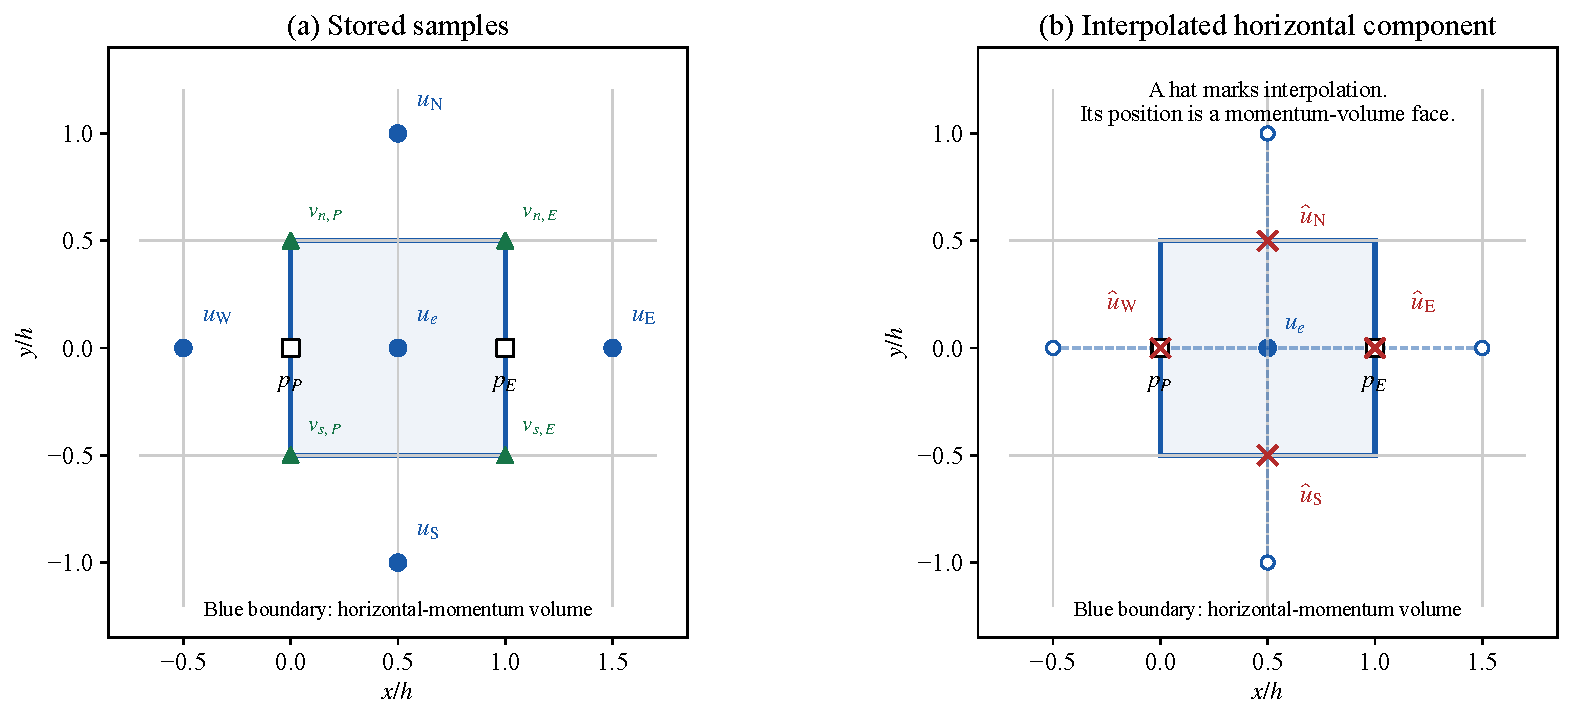
\includegraphics[width=\linewidth]{week01_2_assets/hat_locations.pdf}\end{center}
Use local coordinates with origin at pressure center $P$. The axes are measured in grid spacings $h$. The pressure
centers are $P=(0,0)$ and $E=(h,0)$. The horizontal velocity $u_e$ is stored
at $(h/2,0)$, on their shared pressure-cell face. Its own momentum control
volume is shifted: $0\leq x\leq h$ and $-h/2\leq y\leq h/2$.

The blue circles are stored horizontal components. The red crosses are
evaluation points at the faces of this momentum volume. In these face-flux formulas, a hat denotes
interpolation to a momentum-volume face. The east and west crosses coincide with pressure
centers; the north and south crosses lie at pressure-cell corners. These
geometrical coincidences do not make pressure and horizontal velocity the
same variable.

Each cross lies halfway between two blue samples. For example,
\[
\widehat u_{\rm N}=\frac{u_e+u_{\rm N}}2,\qquad
\widehat u_{\rm E}=\frac{u_e+u_{\rm E}}2.
\]
The subscript N on $u_{\rm N}$ means a neighboring \emph{horizontal} component
one grid spacing to the north. It does not mean a vertical velocity. The green
triangles store vertical components, which supply the speeds carrying fluid
through the north and south faces.

\textbf{Read each mark in its equation.} In the face-flux formulas a hat indicates interpolation; a star indicates
a provisional momentum solution; a prime indicates a pressure or velocity
correction. None of these marks independently identifies a pressure-cell center.
The later PIMPLE equations use $q_{\rm lag}^{(\ell)}$ and
$p_{\rm lag}^{(\ell)}$ for the latest outer-iteration estimates, keeping the hat
for spatial interpolation.
\newpage
\topic{3 continued}{Crossing a face while carrying horizontal momentum}
\begin{center}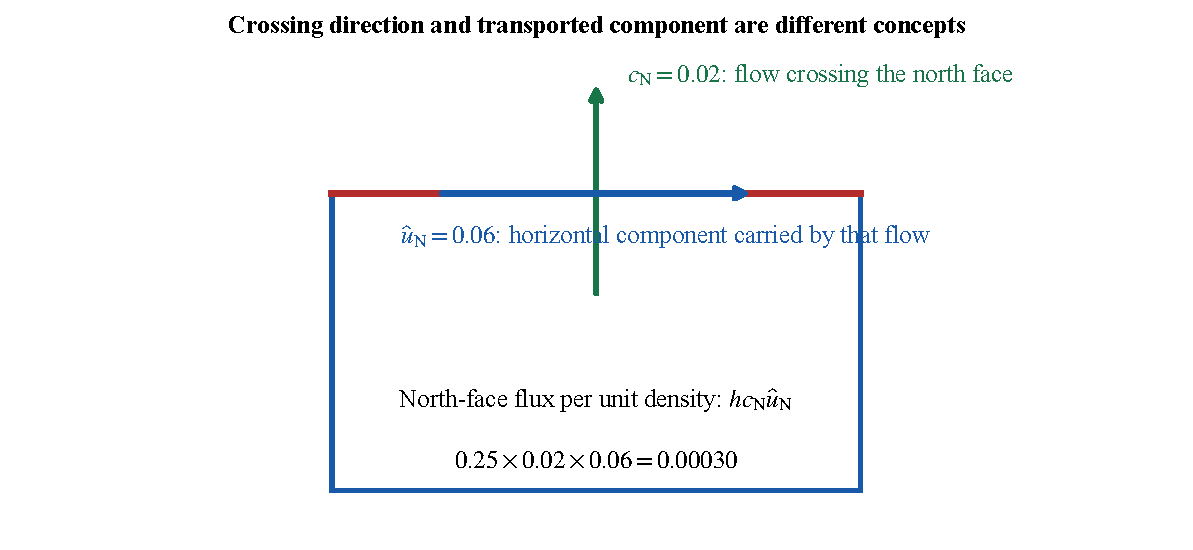
\includegraphics[width=\linewidth]{week01_2_assets/north_face_transport.pdf}\end{center}
At the north face, $c_{\rm N}$ is vertical: it carries fluid across the face.
The transported quantity $\widehat u_{\rm N}$ is horizontal. Per unit density
and unit depth, their product times the face length is the integrated
horizontal-momentum flux $h c_{\rm N}\widehat u_{\rm N}$.

\textbf{Arithmetic example.} Take nondimensional $h=0.25$ and the stored values
\[
(u_e,u_{\rm E},u_{\rm W},u_{\rm N},u_{\rm S})
=(0.04,0.12,0.02,0.08,-0.02).
\]
The four averages are
\[
(\widehat u_{\rm E},\widehat u_{\rm W},\widehat u_{\rm N},\widehat u_{\rm S})
=(0.08,0.03,0.06,0.01).
\]
Let the normal advecting speeds be $(c_{\rm E},c_{\rm W},c_{\rm N},c_{\rm S})
=(0.08,0.03,0.02,0.07)$. The north value averages $v_{n,P}=0.03$ and
$v_{n,E}=0.01$; the south value averages $v_{s,P}=0.05$ and $v_{s,E}=0.09$.
These values also satisfy continuity in the adjacent pressure cells $P$ and $E$.
The momentum volume's outward volume-flux balance is
$h(0.08-0.03+0.02-0.07)=0$. Its horizontal-momentum balance is different:
\begin{align*}
h(c_{\rm E}\widehat u_{\rm E}-c_{\rm W}\widehat u_{\rm W}
+c_{\rm N}\widehat u_{\rm N}-c_{\rm S}\widehat u_{\rm S})
&=0.001600-0.000225+0.000300-0.000175\\
&=0.001500.
\end{align*}
Dividing by area $h^2$ gives the convection term $0.024$. The notebook checks
these values. This is a local interpolation example, not a solved cavity field.

In a linear momentum predictor, advecting speeds $c$ are frozen coefficients;
the transported horizontal components are unknowns. At east and west their
averaging formulas have the same geometry, but their roles in the solve differ.

\newpage
\topic{3 continued}{Central interpolation and face gradients}
In one linear momentum solve, advecting speeds $c$ are evaluated from the
known velocity estimate and then held fixed. This is called freezing the
coefficients. The transported horizontal components remain unknowns. At east and west their
averaging formulas have the same geometry, but their roles in the solve differ.

Let $u_{\rm E},u_{\rm W},u_{\rm N},u_{\rm S}$ be neighboring stored
\emph{horizontal} velocities one grid spacing from $u_e$. They are not the
pressure samples $p_E,p_W,p_N,p_S$. For central interpolation,
\begin{align*}
\widehat u_{\rm E}&=(u_e+u_{\rm E})/2,&
\widehat u_{\rm W}&=(u_{\rm W}+u_e)/2,\\
\widehat u_{\rm N}&=(u_e+u_{\rm N})/2,&
\widehat u_{\rm S}&=(u_{\rm S}+u_e)/2.
\end{align*}
The advecting velocities are obtained from the staggered grid:
\begin{align*}
c_{\rm E}&=(u_e+u_{\rm E})/2,&c_{\rm W}&=(u_{\rm W}+u_e)/2,\\
c_{\rm N}&=(v_{n,P}+v_{n,E})/2,&c_{\rm S}&=(v_{s,P}+v_{s,E})/2.
\end{align*}
For example, $v_{n,P}$ and $v_{n,E}$ are the vertical velocities on the north
faces of pressure cells $P$ and $E$. During a linear momentum solve the $c$
values are held at their current estimates; updating them is a later nonlinear step.

Approximate the gradients at the momentum-volume faces by
\begin{align*}
u_{x,{\rm E}}&\simeq(u_{\rm E}-u_e)/h,&
u_{x,{\rm W}}&\simeq(u_e-u_{\rm W})/h,\\
u_{y,{\rm N}}&\simeq(u_{\rm N}-u_e)/h,&
u_{y,{\rm S}}&\simeq(u_e-u_{\rm S})/h.
\end{align*}
Here $u_{x,{\rm E}}$ means $\partial u/\partial x$ evaluated at the east face.
Substitution and division by $h^2$ turn diffusion into
\[
\beta(u_{\rm E}+u_{\rm W}+u_{\rm N}+u_{\rm S}-4u_e),
\qquad \boxed{\beta=\frac{1}{Re\,h^2}.}
\]
For instance, the east and west contributions combine as
$[(u_{\rm E}-u_e)-(u_e-u_{\rm W})]/(Re\,h^2)$.
The two occurrences of $-u_e$ explain the central $-2u_e$ in that direction.

The full volume-normalized equation is therefore
\begin{align*}
\frac{\mathrm du_e}{\mathrm dt}
&+\frac{c_{\rm E}(u_e+u_{\rm E})-c_{\rm W}(u_{\rm W}+u_e)}{2h}\\
&+\frac{c_{\rm N}(u_e+u_{\rm N})-c_{\rm S}(u_{\rm S}+u_e)}{2h}\\
&=-\frac{p_E-p_P}{h}
+\beta(u_{\rm E}+u_{\rm W}+u_{\rm N}+u_{\rm S}-4u_e).
\end{align*}
Each term has the form of an acceleration. Dividing face length $h$ by
cell area $h^2$ accounts for the factors of $1/h$ in these terms.
\newpage
\topic{3 continued}{Momentum coefficients and numerical example}
For the steady interior row, move each convective neighbor term to the right
and each central diffusive term to the left. Introduce $a_e$ for the coefficient
of the velocity being solved, $a_{\rm E},a_{\rm W},a_{\rm N},a_{\rm S}$ for
its four neighbor coefficients, and $b_e$ for known terms collected on the
right side, such as a prescribed wall-velocity contribution. The result is
\[
\boxed{a_eu_e=a_{\rm E}u_{\rm E}+a_{\rm W}u_{\rm W}
+a_{\rm N}u_{\rm N}+a_{\rm S}u_{\rm S}+b_e-\frac{p_E-p_P}{h}.}
\]
An interior steady row has no time or wall source, so $b_e=0$ there.
The neighbor coefficients are
\begin{align*}
a_{\rm E}&=\beta-c_{\rm E}/(2h),&a_{\rm W}&=\beta+c_{\rm W}/(2h),\\
a_{\rm N}&=\beta-c_{\rm N}/(2h),&a_{\rm S}&=\beta+c_{\rm S}/(2h).
\end{align*}
For example, the east contribution to convection is
$c_{\rm E}u_e/(2h)+c_{\rm E}u_{\rm E}/(2h)$.
The east diffusion term on the right is $\beta u_{\rm E}-\beta u_e$.
Moving terms gives $(\beta-c_{\rm E}/(2h))u_{\rm E}$ on the right and
$(\beta+c_{\rm E}/(2h))u_e$ on the left. Repeating the operation at all faces gives
\begin{align*}
a_e&=4\beta+\frac{c_{\rm E}-c_{\rm W}+c_{\rm N}-c_{\rm S}}{2h}\\
&=a_{\rm E}+a_{\rm W}+a_{\rm N}+a_{\rm S}
+\frac{c_{\rm E}-c_{\rm W}+c_{\rm N}-c_{\rm S}}{h}.
\end{align*}
Do not set the last term to zero merely because the target flow is
incompressible: the current advecting estimates can still have a discrete mass
imbalance. Pressure--velocity coupling removes that imbalance iteratively.
Known wall values contribute to the source and can modify the diagonal.
For a transient problem, the time derivative also supplies a center term and
a known old-time source; those are derived in Section 9.

\textbf{One frozen-row example.} Set $h=0.25$, $Re=100$,
$c_{\rm E}=c_{\rm W}=0.02$, $c_{\rm N}=c_{\rm S}=0$.
Then $\beta=0.16$ and
\[
(a_{\rm E},a_{\rm W},a_{\rm N},a_{\rm S})=(0.12,0.20,0.16,0.16),
\qquad a_e=0.64.
\]
For given neighbor values $(u_{\rm E},u_{\rm W},u_{\rm N},u_{\rm S})
=(0.04,0.02,0.03,0.01)$, their weighted sum is
\[
0.12(0.04)+0.20(0.02)+0.16(0.03)+0.16(0.01)=0.0152.
\]
With $p_P=0.010$, $p_E=0.008$ and $b_e=0$, the pressure contribution is
$-(0.008-0.010)/0.25=+0.008$. Thus
\[
\boxed{u_e=(0.0152+0.008)/0.64=0.03625.}
\]
The lower east pressure drives a positive horizontal contribution.
This satisfies one frozen momentum row; it does not by itself enforce the
neighboring pressure cells' continuity equations. That is the purpose of SIMPLE.
For vertical momentum, apply the same construction around $v_n$; its pressure
term is $-(p_N-p_P)/h$. The next section assembles these scalar rows into a matrix.
